\section{Dimming an LED using PWM}
\subsection{Introduction}
Pulse Width Modulation (PWM) is a technique that allows analog like control over
digital output by controlling the duty cycle of a digital signal.
The level of power depends on the duty cycle, which is the percentage of time
the signal stays on during each cycle.
PWM is commonly used for dimming LEDs and controlling motors.

In STM32F103C6 microcontroller there are several GPIO pins that can 
work as PWM pins. For example the PB0 pin can work as a PWM pin. Using 
the Arduino framework the \texttt{analogWrite} function provides 
the PWM feature. The function takes the pin number and voltage level as the input  and
sends the output voltage according to it.
\subsection{Procedure}
\begin{enumerate}
  \item I have collected a microcontroller STM32 blue pill, STLink programmer,
    a breadboard, an LED, a $220\Omega$ resistor and some jumper wire.
  \item Connected the LED's anode pin to GPIO pin PB0 through the resistor,
    and connected the cathode pin to the ground.
  \item Written the code for dimming the LED (see code~\ref{code:Pushbutton})
    and uploaded it using STLink programmer.
\end{enumerate}
\subsection{Diagram}
\begin{figure}[htbp]
    \centering
\begin{circuitikz}
    \draw 
        (0,0) node[vcc]{PB0} % Power source
        to[R, l=220 $\Omega$] (4,0)
        to[led] (5,0)
        to[short] (6,0)
        to node[sground]{GND} (6,-1);
\end{circuitikz}
\caption{Circuit diagarm for dimming an LED using PWM.}
\label{fig:cir}
\end{figure}
\begin{figure}[htbp]
    \centering
    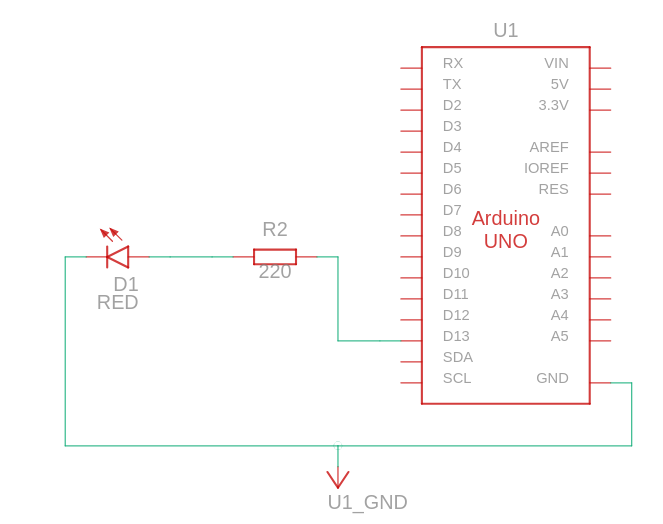
\includegraphics[width=0.5\textwidth]{img/dim-led.png}
    \caption{Schematic diagram of the circuit using Arduino in TinkerCAD}\label{fig:sim}
\end{figure}
\subsection{Source Code}
\begin{code}
\caption{Dimming an LED using PWM in Arduino Framework}
\begin{minted}[frame=single, linenos]{cpp}
#include <Arduino.h>
#define LED_PIN PB0

void setup() { pinMode(LED_PIN, OUTPUT); }

void loop() {
  for (int i = 0; i <= 255; i++) {
    analogWrite(LED_PIN, i);
    delay(10);
  }
  for (int i = 255; i >= 0; i--) {
    analogWrite(LED_PIN, i);
    delay(10);
  }
}
\end{minted}
    \label{code:Pushbutton}
\end{code}

\section{Discussion}
Through this project, I have learned how Pulse Width Modulation (PWM) can be used
to control the brightness of an LED using the STM32F103C6 microcontroller
and the Arduino framework. By varying the duty cycle with the 
\texttt{analogWrite} function,
I understood how digital signals could simulate analog output effectively.
I also gained hands-on experience with setting up hardware connections,
programming with PlatformIO, and working with microcontroller GPIO pins for PWM functionality.
